\documentclass[conference]{IEEEtran}
\usepackage[utf8]{inputenc}
\usepackage{cite}
\usepackage{amsmath,amssymb,amsfonts}
\usepackage{algorithmic}
\usepackage{graphicx}
\usepackage{textcomp}
\usepackage{xcolor}
\usepackage{amsmath}
\usepackage{graphicx}
\usepackage{tikz}
\usepackage{pgfplots}
  \pgfplotsset{compat=newest}
\usepackage{verbatimbox}
\usepackage{interval}
\usepackage{hyperref}
\usepackage{minted}
  \setminted{fontsize=\footnotesize}
  \setminted{breaklines}
  \usemintedstyle{bw}
\newcommand{\code}[1]{\texttt{#1}}
\newcommand{\nospell}[1]{#1}
\newenvironment{nicetable}
  {\setlength{\parindent}{0em}\medskip\small}
  {\medskip}
\begin{document}
\title{The Impact of Constructors on the Validity of Class Cohesion Metrics}
\author{Yegor Bugayenko\\
Huawei Technologies Co., Ltd.\\
Russian Research Institute,\\
Moscow, Russia\\
yegor.bugayenko@huawei.com}

\maketitle

\begin{abstract}
Class cohesion is a measure of the degree to which a class's
inner elements, like methods and attributes, are bound or related
to one another. There have been over thirty different formulas proposed in order to
calculate the metric. None of them are explicitly designed to
deal with constructors in any different way than with regular methods---they
simply treat them as identical entities.
However, as many object-oriented theorists say, constructors
play a very specific role in object life-cycle. In the scope of this empirical
research, five different formulas were implemented in two ways: including
constructors and excluding them. Then both set of formulas were applied to
the same set of 1000 mid-size open source Java projects. The results obtained demonstrated
how much of a distraction constructors were bringing into metric calculations.
\end{abstract}

%%%%%%%%%%%%%%%%%%%%%%%%%%%%%%%%%%%%%%%%%%%%%%%%%%%%%%%%%%%%%%%%%%%%%%%%%%%%%%%%%%%%%%%%%%%%%%%%%%%%%%%%%%%%%%%%%%%%%%%
%%%%%%%%%%%%%%%%%%%%%%%%%%%%%%%%%%%%%%%%%%%%%%%%%%%%%%%%%%%%%%%%%%%%%%%%%%%%%%%%%%%%%%%%%%%%%%%%%%%%%%%%%%%%%%%%%%%%%%%
%%%%%%%%%%%%%%%%%%%%%%%%%%%%%%%%%%%%%%%%%%%%%%%%%%%%%%%%%%%%%%%%%%%%%%%%%%%%%%%%%%%%%%%%%%%%%%%%%%%%%%%%%%%%%%%%%%%%%%%
\section{Introduction}

Class cohesion, as a degree of ``how tightly bound or related its internal
elements are to one another,''~\cite{yourdon78}
is considered as one of the most important object-oriented software
attributes~\cite{badri08,yourdon78,kabaili01}.
A class with low cohesion has disparate and non-related members;
cohesion can be used to identify the poorly designed classes~\cite{badri08,basili96,chowdhury11}.

There are over thirty different metrics introduced so far to
measure functional~\cite{dhama95,bieman95} cohesion of a class~\cite{izadkhah17,dallal10}.
All of them in one way or the other analyze
the amount and the structure of class attributes and methods in order to calculate the
metric. Almost none of them, however, explicitly mention in their
descriptions whether constructors should be treated as methods or
whether they have to have a special status.

From a theoretical standpoint, constructors and methods play very different
roles in the life-cycle of an object~\cite{west04}. This fundamental difference between
them must affect class cohesion in some way. The assumption is that excluding
constructors from formulas will make these formulas produce more
meaningful and reasonable results.

%%%%%%%%%%%%%%%%%%%%%%%%%%%%%%%%%%%%%%%%%%%%%%%%%%%%%%%%%%%%%%%%%%%%%%%%%%%%%%%%%%%%%%%%%%%%%%%%%%%%%%%%%%%%%%%%%%%%%%%
%%%%%%%%%%%%%%%%%%%%%%%%%%%%%%%%%%%%%%%%%%%%%%%%%%%%%%%%%%%%%%%%%%%%%%%%%%%%%%%%%%%%%%%%%%%%%%%%%%%%%%%%%%%%%%%%%%%%%%%
%%%%%%%%%%%%%%%%%%%%%%%%%%%%%%%%%%%%%%%%%%%%%%%%%%%%%%%%%%%%%%%%%%%%%%%%%%%%%%%%%%%%%%%%%%%%%%%%%%%%%%%%%%%%%%%%%%%%%%%
\section{Constructors' Mission}

Most object-oriented publications, both scientific and practical, pay
a relatively small amount of attention to object constructors
in comparison to methods, attributes, types, and other ingredients
of object-oriented design.
For example, \emph{Clean Code}~\cite{martin08} and \emph{Refactoring}~\cite{fowler99},
rather popular books about object-oriented programming,
have no special sections or even paragraphs giving an explanation
of what constructors are for and what is important in their design.
The book \emph{Object-Oriented Software Construction}\cite{meyer97}
mentions the word ``constructor'' just nine times through almost 1300 pages of text,
calling them ``creation procedures of a class,'' and providing almost
no additional information.
\emph{The C++ Programming Language}~\cite{stroustrup13} says that constructors are
``member functions\ldots that define a way to initialize an object of its class,''
adding no recommendations or discussions for their design.
\emph{Growing Object-Oriented Software}~\cite{freeman09}
has a single side note about constructors, which says that
``our experience is that busy constructors enforce assumptions that one day we will
want to break, especially when testing, so we prefer to keep them very
simple—just setting the fields,'' and that was the only thought dedicated to
constructors in the entire book.
\emph{Object-Oriented Analysis and Design}~\cite{booch07}
calls constructors at the same time ``member functions,''
``operations,'' and ``\nospell{metaoperations},'' saying that their basic responsibility
is ``to create an instance of the class and populate it
with a set of rules, which it then uses for evaluation,''
but does not develop the discussion in any further direction.

Most modern object-oriented programming languages, like Ruby, Python or PHP
technically don't differentiate constructors and regular object methods---they
just call certain methods by names, which are selected by convention, e.g.
\code{initialize()} in Ruby or \code{\_\_construct()} in PHP.
Smalltalk doesn't have constructors at all~\cite{goldberg83}.

It seems that constructors, information-wise, are treated as second class citizens;
there is obviously a lack of attention to them in academic and professional publications.
In most places, including in the formulas of cohesion metrics,
which will be demonstrated further, there is no distinction being drawn between
them and regular methods.

This doesn't seem right, however, since the nature of constructors is different from the nature of object methods.
First, constructors are not intended to do any work, but must only initialize object attributes~\cite{bugayenko16}.
Second, they (by definition) must ``touch'' all attributes in order to initialize them,
or call other constructors that do that job; some languages---like Kotlin or Scala~\cite{odersky14}---make
this separation of primary and secondary constructors explicit and mandatory.
Third, they always ``return'' the same object type~\cite{bloch18}.
Forth, they are always present in any object, either explicitly or synthetically generated by the compiler.
At least because of these differences, applying the same design ``best practices'' to them as to regular methods
seems to be a flawed idea.
The empirical analysis performed below demonstrates that this concern has its grounds.

%%%%%%%%%%%%%%%%%%%%%%%%%%%%%%%%%%%%%%%%%%%%%%%%%%%%%%%%%%%%%%%%%%%%%%%%%%%%%%%%%%%%%%%%%%%%%%%%%%%%%%%%%%%%%%%%%%%%%%%
%%%%%%%%%%%%%%%%%%%%%%%%%%%%%%%%%%%%%%%%%%%%%%%%%%%%%%%%%%%%%%%%%%%%%%%%%%%%%%%%%%%%%%%%%%%%%%%%%%%%%%%%%%%%%%%%%%%%%%%
%%%%%%%%%%%%%%%%%%%%%%%%%%%%%%%%%%%%%%%%%%%%%%%%%%%%%%%%%%%%%%%%%%%%%%%%%%%%%%%%%%%%%%%%%%%%%%%%%%%%%%%%%%%%%%%%%%%%%%%
\section{Five Cohesion Metrics}

There are over thirty different metrics existing to measure
class cohesion~\cite{izadkhah17}. A few of them were selected
for the experiment:

The Normalized Hamming Distance (\textbf{NHD}) class cohesion metric
measures the similarity in all methods of a class in terms of
the types of their arguments~\cite{counsell06}. Let $l$ be the number of
distinct parameter types, $k$ be the number of methods,
and $c_j$ be the number of methods that have a parameter of type $j$,
then,

\begin{equation}
\mathit{NHD} = 1 - \frac{2}{lk(k-1)} \sum_{j=1}^{l} c_j(k-c_j).
\end{equation}

The Sensitive Class Cohesion Metric (\textbf{SCOM}) is a
ratio of the sum of connection intensities $C_{i,j}$ of
all pairs $(i,j)$ of $m$ methods to the total number of pairs of methods.
Connection intensity must be given more weight $\alpha_{i,j}$ when such a
pair involves more attributes~\cite{fernandez06}:

\begin{equation}
\mathit{SCOM} = \frac{2}{m(m-1)} \sum_{i=1}^{m-1} \sum_{j=i+1}^{m} C_{i,j} \times \alpha_{i,j}
\end{equation}

The Method-Method through Attributes Cohesion (\textbf{MMAC}) metric is
the average cohesion of all pairs of methods\cite{dallal07}.
Let $k$ be the number of methods, $l$ be the number of distinct parameter types,
and $x_i$ be the number of methods that use type $i$, then

\begin{equation}
\mathit{MMAC} = \frac{1}{lk(k-1)} \displaystyle\sum_{i=1}^{l} x_i (x_i - 1).
\end{equation}

The Cohesion Among Methods in Class (\textbf{CAMC})
measures the extent of intersections of individual method parameter
type lists with the parameter type list of all methods in the class~\cite{bansiya99}.
Let $l$ be the number of distinct parameter types, $k$ be the number
of methods and $p_i$ be the number of distinct parameter
types used by method $i$, then

\begin{equation}
\mathit{CAMC} = \frac{1}{lk} \sum_{i=1}^{k} p_i.
\end{equation}

The Lack of Cohesion of Methods (\textbf{LCOM}) is
a correlation between the methods and the local instance variables of a class
(we use the version suggested by \cite{henderson96}, also known as LCOM5).
Let $m$ be the number of methods, $a$ be the number of
attributes and $\mu_j$ be the amount of methods, which use attribute $j$, then

\begin{equation}
\mathit{LCOM} = \frac{1}{1 - m} \left( \dfrac{1}{a} \displaystyle\sum_{j=1}^{a} \mu_j \right) - m.
\end{equation}

For all metrics, except LCOM, greater values mean higher cohesion. The LCOM
metric is reversed and demonstrates smaller values for higher cohesion. In order
to make the discussion easier we use the inverted version of this metric,
which is:

\begin{equation}
\mathit{LCOM} = 1 - \mathit{LCOM}.
\end{equation}

The values of all metrics are in the $\interval{0}{1}$ interval.

Even though it would be beneficial for this experiment to use all or most
of the available metrics, this is not technically feasible for a number
of reasons. First, the implementation of each metric takes a certain amount of time to understand
the formula, implement the algorithm in Java, and make sure it works as intended
(at least 80 work hours).
Second, some metrics were suggested by their authors without a thorough testing
with all possible Java code samples. In other words, they work in theory
but can't be implemented ``as is'' in practice, while adapting their
algorithms to the reality of Java code may break their integrity and compromise the
original idea of their authors. The metrics used in this research are implemented
exactly as they were suggested by their authors and they work correctly with
all available Java classes.

%%%%%%%%%%%%%%%%%%%%%%%%%%%%%%%%%%%%%%%%%%%%%%%%%%%%%%%%%%%%%%%%%%%%%%%%%%%%%%%%%%%%%%%%%%%%%%%%%%%%%%%%%%%%%%%%%%%%%%%
%%%%%%%%%%%%%%%%%%%%%%%%%%%%%%%%%%%%%%%%%%%%%%%%%%%%%%%%%%%%%%%%%%%%%%%%%%%%%%%%%%%%%%%%%%%%%%%%%%%%%%%%%%%%%%%%%%%%%%%
%%%%%%%%%%%%%%%%%%%%%%%%%%%%%%%%%%%%%%%%%%%%%%%%%%%%%%%%%%%%%%%%%%%%%%%%%%%%%%%%%%%%%%%%%%%%%%%%%%%%%%%%%%%%%%%%%%%%%%%
\section{Research Method and Results}

The most popular place for publishing open source Java artifacts
is Maven Central Repository~\cite{miller10}.
There were 35211 artifacts found,%
\footnote{\url{https://github.com/yegor256/scrape-maven-central}}
which released at least one version in 2017.
Even though such a large data set constitutes a perfect analysis corpus,
it was decided to use only a subset of the entire Maven Central Repository.
The main reason behind this decision was the amount of time
and computing resources required for the analysis of a single
Java artifact: 100-500 seconds (more than 100 days for the entire Maven Central).

Artifacts with less than one hundred or more than two thousand
\code{.class} files were filtered out.
926 artifacts remained in the list.
This size-based selection criteria was selected due to the following
assumptions: 1) artifacts with fewer classes may represent
abnormally better design due to the attention their developers
were able to pay to each individual class, 2) artifacts with a lot
of classes may represent the opposite situation, where developers
didn't have enough time to pay attention to the quality of design.
To exclude these abnormalities it was decided to exclude too big
and too small artifacts and analyze only mid-sized ones.

Cohesion metrics were implemented in the scope of jPeek,
an open source Java command line utility and a web system.%
\footnote{\url{https://github.com/yegor256/jpeek}}
jPeek parses Java bytecode \code{.class} files via Javassist~\cite{chiba98},
analyzes its internals with the help of ASM~\cite{bruneton02},
and then creates an XML representation of the entire artifact,
where each class is presented by an XML element.

Interfaces, annotations, enums, anonymous classes,
and classes generated by the AspectJ aspect-oriented
framework were filtered out, because none of them represent
actual objects in terms of object-oriented design. They are either
auto-generated or surrogates (like enums).

For example, take a simple Java class:

\begin{minted}{text}
class Book {
  private int id;
  int getId() {
    return this.id;
  }
}
\end{minted}

It would be represented by jPeek in the output XML file as follows:

\begin{minted}{text}
<class id='Book'>
  <attributes>
   <attribute public='false' static='false' type='I'>id</attribute>
  </attributes>
  <methods>
    <method abstract='false' ctor='false' desc='()I' name='getId' public='true' static='false'>
      <return>I</return>
      <args/>
    </method>
  </methods>
</class>
\end{minted}

Next, metric-specific XSL transformations~\cite{kay00} were applied to the XML file
in each artifact, in order to generate measurements for each metric.
For example, MMAC metric produced this XML file in
the \code{org.mockito:mockito-all} artifact:

\begin{minted}{text}
<metric>
  <title>MMAC</title>
  <app>
    <class id='InstantiatorProvider' value='1'/>
    <class id='InstantationException' value='0'/>
    <class id='AnswersValidator' value='0.0583'/>
    <class id='ClassNode' value='0.25'/>
    [... skipped ...]
  </app>
</metric>
\end{minted}

Here, \code{AnswersValidator} and \code{ClassNode} are class names,
while \code{0.0583} and \code{0.25} are their corresponding values of
the MMAC formula, referred to below as $v(c,m,a)$, where
$c$ is the class, $m$ is the metric, and $a$ is the Java artifact.

Next, the minimum and the maximum of all $v$ in each XML file were found.
For example, in \code{MMAC.xml} they were 0 and 1 respectively, for the Mockito
artifact mentioned above. Then, all classes, which
demonstrated values equal to either minimum or maximum, were filtered out. This was done in order
to minimize the influence of trivial classes, which most of the Java artifacts
contain. For example, most metrics would consider this class as highly cohesive
or even ``perfect,'' despite its very low usefulness:

\begin{minted}{text}
class Book {
  // The body of the class is empty,
  // no attributes, no methods.
}
\end{minted}

Since most Java artifacts contain classes of a similarly trivial kind, it was considered
reasonable to filter our highest and lowest values, to reduce noise.
It was
observed that some libraries have many classes with maximum or minimum metric
values. The investigation of more than a hundred of them showed that
all of them are either 1) empty classes with no methods and no attributes,
or 2) utility classes with a large amount of static methods and no attributes.

Then, the arithmetic mean $\mu_{m,a}$ was calculated for a set of all
$N$ measurements $v(1,m,a), v(2,m,a),\dots, v(N,m,a)$ as:

\begin{equation}
\mu_{m,a} = \frac{1}{N}\sum_{i=1}^N v(i,m,a).
\end{equation}

Then, the standard deviation $\sigma_{m,a}$ was calculated as:

\begin{equation}
\sigma_{m,a} = \sqrt{\frac{1}{N}\sum_{i=1}^N (v(i,m,a) - \mu_{m,a})^2}.
\end{equation}

It was observed that even though most artifacts demonstrated rather
small values of $\sigma$ (within one standard deviation of $\mu$,
or about 32\%), in some of them
the distribution of values was far from normal (normality checks were performed to test this fact).
It was decided to filter out artifacts which had $\sigma$ values larger than
one standard deviation, in order to focus on artifacts where classes
are designed with the highest uniformity.
100 artifacts remained in the list.

Thus, after the described calculations, the entire list of Java artifacts produced
the matrix of $\mu_{m,a}$, where $m$ values are columns and $a$
values are rows, as shown in the Table~\ref{tab:1}.

\begin{table}[h]
  \caption{Metrics calculated per each artifact}
  \begin{nicetable}
  \begin{tabular}{\nospell{lrrrrr}}
  \hline
  % nothing
    & \rotatebox[origin=c]{90}{NHD}
    & \rotatebox[origin=c]{90}{SCOM}
    & \rotatebox[origin=c]{90}{MMAC}
    & \rotatebox[origin=c]{90}{CAMC}
    & \rotatebox[origin=c]{90}{LCOM} \\
  \hline
  \code{io.vavr:vavr} & 0.31 & 0.59 & 0.47 & 0.55 & 0.31 \\
  \code{xerces:xercesImpl} & 0.78 & 0.51 & 0.30 & 0.33 & 0.14 \\
  \code{org.takes:takes} & 0.21 & 0.44 & 0.38 & 0.87 & 0.32 \\
  \code{com.h2database:h2} & 0.75 & 0.73 & 0.18 & 0.44 & 0.17 \\
  \dots \\
  \hline
  \end{tabular}
  \label{tab:1}
  \end{nicetable}
\end{table}

Next, a ranking formula was introduced, in order to calculate the
position of each particular artifact $a$ in the entire set. Artifact rank $r_a$
was calculated as an arithmetic average of all $\mu_{m,a}$ values in all
$M$ metrics:

\begin{equation}
r_a = \frac{1}{M}\sum_{j=1}^{M} \mu_{j,a}.
\end{equation}

Thus, the entire list of artifacts was sorted by artifact ranks $r_a$. Each
artifact got its own position $p_a$ in the list.

Then class cohesion formulas were modified, in order to exclude constructors
from calculations, and all artifacts were ranked again and re-ordered. Ergo, two
ordered lists of artifacts were created. The first one, where all formulas
treated constructors as regular methods; and the second one, where constructors
were excluded. The position of the artifact $a$ in the first list is denoted as $p_a$,
while the position of the same artifact in the second list is $p'_a$.

Then, the differences between $p_a$ and $p'_a$ were calculated, in order to
understand how big the effect of constructor removal is and whether the
effect has an obvious tendency:

\begin{equation}
d_a = p_a - p'_a.
\end{equation}

The $d_a$ numbers obtained are presented in the Figure~\ref{fig:1}, where
horizontal axis is the value of $d_a$ and the vertical axis is the amount of
classes in the artifact.

\begin{figure}[h]
  \caption{Differences between artifact positions, with constructors and without them}
  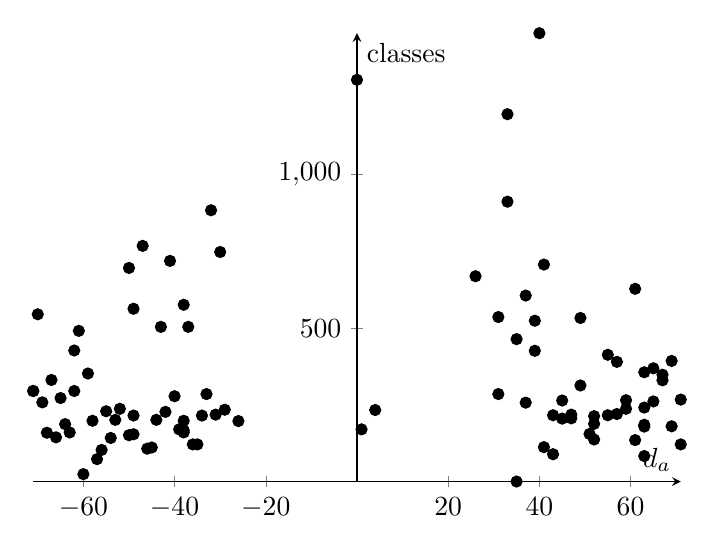
\begin{tikzpicture}
  \begin{axis}[axis lines=middle, xlabel=$d_a$, ylabel={classes}, x post scale=1.2,xmin=-71, xmax=71, ymin=0, ymax=1461]
  \addplot [only marks] table {
  0 1309
  63 356
  71 267
  69 393
  67 348
  65 261
  63 179
  61 135
  59 265
  57 390
  55 413
  52 213
  63 83
  49 533
  47 218
  45 264
  43 89
  41 112
  39 426
  37 606
  35 464
  33 912
  31 536
  51 155
  52 188
  26 669
  63 185
  71 121
  69 180
  67 330
  65 369
  63 241
  61 628
  59 237
  57 220
  55 216
  52 137
  40 1461
  49 313
  47 206
  45 205
  43 216
  41 707
  39 524
  37 257
  35 0
  33 1197
  31 285
  4 233
  1 170
  -49 563
  -38 198
  -30 748
  -32 884
  -34 215
  -36 121
  -38 167
  -40 278
  -42 227
  -44 201
  -46 107
  -49 154
  -38 576
  -52 237
  -54 142
  -56 103
  -58 198
  -60 24
  -62 427
  -64 187
  -66 144
  -68 159
  -70 545
  -50 151
  -49 215
  -26 197
  -38 160
  -29 234
  -31 218
  -33 285
  -35 121
  -37 504
  -39 170
  -41 719
  -43 504
  -45 111
  -47 768
  -50 696
  -62 295
  -53 201
  -55 229
  -57 73
  -59 352
  -61 491
  -63 160
  -65 272
  -67 331
  -69 258
  -71 295
  -71 295
  };
  \end{axis}
  \end{tikzpicture}
  \label{fig:1}
\end{figure}

The distribution of numbers is visibly wide, taking into account the amount
of items in the list: one hundred. This means that for many of them the position
$p_a$ has been changed significantly---most of the numbers $d_a$ are grouped
around +50 and -50. This means that the exclusion of constructors changed
the essence of the opinions the metrics were giving about the artifacts provided.
Highly cohesive classes became very \nospell{uncohesive} and vice versa.

%%%%%%%%%%%%%%%%%%%%%%%%%%%%%%%%%%%%%%%%%%%%%%%%%%%%%%%%%%%%%%%%%%%%%%%%%%%%%%%%%%%%%%%%%%%%%%%%%%%%%%%%%%%%%%%%%%%%%%%
%%%%%%%%%%%%%%%%%%%%%%%%%%%%%%%%%%%%%%%%%%%%%%%%%%%%%%%%%%%%%%%%%%%%%%%%%%%%%%%%%%%%%%%%%%%%%%%%%%%%%%%%%%%%%%%%%%%%%%%
%%%%%%%%%%%%%%%%%%%%%%%%%%%%%%%%%%%%%%%%%%%%%%%%%%%%%%%%%%%%%%%%%%%%%%%%%%%%%%%%%%%%%%%%%%%%%%%%%%%%%%%%%%%%%%%%%%%%%%%
\section{Conclusion}

First, the observed effect of constructor removal from the formulas of the five class cohesion metrics
confirms that constructors can't be treated similarly
to regular methods. They play a different role in object design and must find their own place
in existing formulas or some new formulas have to be introduced.

Second, a more detailed individual analysis of the effect
constructor removal had on a few selected classes from a few
Java open source artifacts, made it obvious that a larger number
of constructors does not make a class less cohesive, despite the
opinion all analyzed metrics showed.

\section{Acknowledgements}

The author is thankful to the contributors who
helped design and implement jPeek open source Java software, including,
but not limited to (in alphabetic order):
\nospell{Mihai Andronache},
\nospell{George Aristy},
\nospell{Sergey Kapralov},
\nospell{Sergey Karazhenets},
\nospell{Paulo Lobo},
\nospell{Vladimir Motsak},
\nospell{Alonso A. Ortega},
\nospell{Rok Pov\v{s}i\v{c}},
\nospell{Vseslav Sekorin},
\nospell{Mehmet Yildirim}.

\begin{thebibliography}{}
\nospell{

\bibitem{aggarwal06}
K. K. Aggarwal,
\emph{Empirical Study of Object-Oriented Metrics},
Journal of Object Technology, Volume~5, Number~8, 2006.

\bibitem{badri08}
L. Badri et al.,
\emph{Revisiting Class Cohesion: An empirical investigation on several systems},
Journal of Object Technology, Volume~7, Number~6, 2008.

\bibitem{bansiya99}
J. Bansiya et al.,
\emph{A class cohesion metric for object-oriented designs},
Journal of Object-Oriented Programming,
Volume~11, Number~8, 1999.

\bibitem{basili96}
V. R. Basili et al.,
\emph{A validation of object-oriented design metrics as quality indicators},
IEEE Transactions on Software Engineering, Volume~22, Issue~10, 1996.

\bibitem{bloch18}
J. Bloch,
\emph{Effective Java},
Addison-Wesley Professional, 3rd edition, 2018.

\bibitem{bruneton02}
E. Bruneton et al.,
\emph{ASM: a code manipulation tool to implement adaptable systems},
Adaptable and extensible component systems, 30(19), 2002.

\bibitem{booch07}
G. Booch et al.,
\emph{Object-Oriented Analysis and Design with Applications},
Addison-Wesley Professional, 3rd edition, 2007.

\bibitem{bugayenko16}
Y. Bugayenko,
\emph{Elegant Objects},
Volume~1, Create Space, 2016.

\bibitem{chiba98}
S. Chiba,
\emph{Javassist---A Reflection-based Programming Wizard for Java},
Proceedings of OOPSLA'98 Workshop on Reflective Programming in C++ and Java, Volume~174, 1998.

\bibitem{chowdhury11}
I. Chowdhury et al.,
\emph{Using complexity, coupling, and cohesion metrics as early indicators of vulnerabilities},
Journal of Systems Architecture, Volume~57, Issue~3, 2011.

\bibitem{counsell06}
S. Counsell et al.,
\emph{The interpretation and utility of three cohesion metrics for object-oriented design},
ACM Transactions on Software Engineering and Methodology (TOSEM),
Volume~15, Issue~2, 2006.

\bibitem{dallal07}
J. A. Dallal,
\emph{A Design-Based Cohesion Metric for Object-Oriented Classes},
International Journal of Computer and Information Engineering,
Volume~1, Number~10, 2007.

\bibitem{dallal10}
J. A. Dallal,
\emph{Mathematical Validation of Object-Oriented Class Cohesion Metrics},
International Journal of Computers, Issue~2, Volume~4, 2010.

\bibitem{dhama95}
H. Dhama,
\emph{Quantitative models of cohesion and coupling in software},
Journal of Systems and Software,
Volume~29, Issue~1, 1995.

\bibitem{fernandez06}
L. Fern\'andez et al.,
\emph{A Sensitive Metric of Class Cohesion},
International Journal ``Information Theories \& Applications'',
Volume 13, 2006,

\bibitem{fowler99}
M. Fowler,
\emph{Refactoring: Improving the Design of Existing Code},
Addison-Wesley Professional, 1999.

\bibitem{fowler02}
M. Fowler,
\emph{Patterns of Enterprise Application Architecture},
Addison-Wesley Professional, 2002.

\bibitem{freeman09}
S. Freeman et al.,
\emph{Growing Object-Oriented Software, Guided by Tests},
Addison-Wesley Professional, 2009.

\bibitem{gamma94}
E. Gamma et al.,
\emph{Design Patterns: Elements of Reusable Object-Oriented Software},
Addison Wesley, 1994.

\bibitem{goldberg83}
A. Goldberg,
\emph{Smalltalk-80: The Language and its Implementation},
Addison-Wesley, 1983.

\bibitem{henderson96}
B. Henderson-Sellers et al.,
\emph{Coupling and cohesion (towards a valid metrics suite for object-oriented analysis and design)},
Object Oriented Systems, Volume~3, Number~3, 1996.

\bibitem{izadkhah17}
H. Izadkhah et al.,
\emph{Class Cohesion Metrics for Software Engineering: A Critical Review},
Computer Science Journal of Moldova, Volume~25, Number~1(73), 2017.

\bibitem{kabaili01}
H. Kabaili,
\emph{Cohesion as changeability indicator in object-oriented systems},
Proceedings Fifth European Conference on Software Maintenance and Reengineering, 2001.

\bibitem{kay00}
M. Kay,
\emph{XSLT Programmer's Reference},
Wrox Press, 2000.

\bibitem{martin08}
R. C. Martin,
\emph{Clean Code: A Handbook of Agile Software Craftsmanship},
Prentice Hall, 2008.

\bibitem{meyer97}
B. Meyer,
\emph{Object-Oriented Software Construction},
Prentice Hall, 2nd edition, 1997.

\bibitem{miller10}
F. P. Miller et al.,
\emph{Apache Maven},
Alpha Press, 2010

\bibitem{odersky14}
M. Odersky,
\emph{The Scala Language Specification},
EPFL, 2014.

\bibitem{stroustrup13}
B. Stroustrup,
\emph{The C++ Programming Language},
Addison-Wesley Professional, 4th edition, 2013.

\bibitem{west04}
D. West,
\emph{Object Thinking},
Microsoft Press, 2004.

\bibitem{yourdon78}
E. Yourdon et al.,
\emph{Structured Design: Fundamentals of a Discipline of Computer Program and Systems Design},
2nd Edition, Yourdon Press, 1978.

\bibitem{bieman95}
J. M. Bieman,
\emph{Cohesion and reuse in an object-oriented system},
Proceedings of the 1995 Symposium on Software, 1995.
}

\end{thebibliography}
\end{document}
